\documentclass[pdflatex]{sn-jnl}
\jyear{2024}
\usepackage{multibib}
\newcites{m}{Methods References}
\usepackage[superscript]{cite}
\usepackage{caption}
\bibliographystyle{unsrt}
\bibliographystylem{unsrt} 
\raggedbottom

% Remove numbering from sections and subsections, as requested in decision email.
\setcounter{secnumdepth}{0}


\newcommand{\yohai}[1]{{\textcolor{red}{#1}}}
\newcommand{\neri}[1]{{\textcolor{cyan}{#1}}}


\begin{document}

\title[Running Title]{Does an earthquake “know” how big it will be? A neural-net aided study} % 2nd option: Using past seismicity to predict the magnitude of future earthquakes

\author[1,2]{\fnm{Neri} \sur{Berman}}\email{neriberman@gmail.com}
\author[2]{\fnm{Oleg} \sur{Zlydenko}}
\author[2]{\fnm{Oren} \sur{Gilon}}
\author[1]{\fnm{Yohai} \sur{Bar-Sinai}}\email{ybarsinai@gmail.com}

\affil[1]{\orgdiv{Department of Physics}, \orgname{Tel-Aviv University}, \orgaddress{\city{Tel-Aviv}, \country{Israel}}}
\affil[2]{\orgdiv{Google Research}, \orgname{Google}, \orgaddress{\city{Tel-Aviv}, \country{Israel}}}


\abstract{
Earthquake occurrence is notoriously difficult to predict. Salient features of their spatiotemporal statistics can be relatively well captured by point-process models \neri{this is mentioning ETAS. But it is also not completely true. We should remove the mention of PP IMO}. However, very little is known regarding the magnitude of future events, and it is deeply debated whether it is possible to predict the magnitude of an earthquake before it starts, both due to the lack of information about fault conditions and to the inherent complexity of rupture dynamics. Consequently, even state of the art forecasting models typically assume no knowledge about the magnitude of future events besides the time-independent Gutenberg Richter distribution, which describes the marginal distribution over large regions and long times. This approach implicitly assumes that earthquake magnitudes are independent of seismic history and are identically distributed. In this work we challenge this view by showing that information about the magnitude of an upcoming earthquake can be directly extracted from the seismic history. We present a neural network-based model for probabilistic forecasting of future magnitudes based on cataloged properties: hypocenter locations, occurrence times and magnitudes of past earthquakes. Our history-dependent model outperforms stationary and quasi-stationary state of the art GR-based benchmarks, in real catalogs in Southern California, Japan and New-Zealand.  This demonstrates that earthquake catalogs contain information about the magnitude of future earthquakes, prior to their occurrence. We conclude by proposing methods to apply the model in characterization of the preparatory phase of earthquakes, and in operational hazard alert and earthquake forecasting systems.
}

\keywords{}

\maketitle

\neri{comment by Neri} \newline
\yohai{comment by Yohai}


\section{Introduction} \label{sec:introduction}
Earthquakes are notoriously unpredictable, and forecasting seismicity is a long-standing scientific and technological challenge, often deemed unrealistic due to the inherent complexity of earthquake processes and the scarcity of near-field data~\cite{bernard_earthquake_1999, geller_earthquakes_1997}. 
Research since the late 19th century has provided much phenomenological insight about the spatiotemporal statistics of earthquakes, including various marginal distributions \cite{gutenberg_frequency_1944, kagan_seismic_2002}, scaling relations \cite{bak_earthquakes_1989, dascher-cousineau_what_2020, kagan_aftershock_2002, utsu_centenary_1995} and characteristics of both spatial and temporal clustering \cite{omori_after-shocks_1894, kagan_short-term_2004, ben-zion_localization_2020, devries_deep_2018, king_static_1994}. Clearly, these insights can be used to quantitatively inform us about future seismicity based on recent history. For example, Omori's law tells us that after big earthquakes we should expect an increase in the local seismicity rate~\cite{omori_after-shocks_1894}. Such laws have been incorporated into a variety of forecasting models, which are operationally used today\cite{ogata_statistical_1988, hardebeck_aftershock_2024, jordan_operational_2011, stirling_national_2012}.

However, the above mentioned statistical relations only describe the rate and locations of earthquakes, and very little is known about the dependence of earthquake magnitude on seismic history.
It is deeply debated whether it is possible to determine the magnitude of an earthquake before it starts~\cite{kagan_seismic_2002, ogata_exploring_2018}, or even during rupture~\cite{ellsworth_seismic_1995, meier_evidence_2016}.
Most modeling approaches assume that event magnitudes follow and identical and independent stationary (or almost stationary) distribution - the Gutenberg Richter distribution (GR), which describes the marginal magnitude distribution over large regions and long times. 
While some variations in magnitude statistics have been described \cite{gulia_real-time_2019, nandan_magnitude_2019}, they all model history dependence by weak and slow changes in the parameters of the GR distribution, and do not model the magnitude of \textit{a specific} future event. Operationally, state-of-the-art forecasting models typically assume no knowledge about the magnitude of future events besides the marginal GR distribution, an assumption known as separability \cite{schoenberg_testing_2004}. Namely, the separability assumption is that the distribution of earthquake magnitudes is statistically independent of the distribution of earthquakes locations and times.

This modeling approach is not a naive or uninformed choice.  Current research on magnitude prediction has failed to show a universal and reproducible advantage over a stationary or quasi-stationary GR benchmark~\cite{ogata_exploring_2018, stockman_forecasting_2023}. Indeed, due to the spatial complexity of the elastic fields, faulting patterns and lithology, the nonlinearities of the rupture process and the complicated interaction between them all, it is not far-fetched to assume that determining the magnitude of an event requires a detailed microscopic knowledge of the system's state. 
This philosophy also inspired physical models which describe earthquake dynamics with a statistical approach \cite{olami_self-organized_1992, sornette_self-organized_1989, bak_earthquakes_1989, de_geus_scaling_2022}. These models reproduce many of the phenomenological statistical relations by positing that faults evolve (``self-organize'') towards a critical state, where events emerge stochastically and their magnitude follows a power-law distribution which is scale-free and self-similar, akin to physical systems in the vicinity of a phase transition. Under this paradigm, determining the magnitude of an event is indeed impossible using only far-field measurements. 

Previous studies have not identified a definitive link between earthquake magnitude and seismic history \cite{petrillo_verifying_2023}\neri{More citations needed}. Research focused on predicting future earthquake magnitudes often explores questions distinct from those addressed here. While some have yielded interesting results, the absence of comparisons to established benchmarks \cite{shcherbakov_forecasting_2019, panakkat_neural_2007} hinders objective assessment of their efficacy and progress. Other studies specifically targeting magnitude prediction have yet to outperform the GR distribution \cite{stockman_forecasting_2023}. Thus, previous studies have not yet systematically shown the ability to extract meaningful information from seismic history beyond what a random selection from the GR distribution would provide. Consequently, the question regarding the dependence of magnitude on seismic history remains open.

The main goal of this paper is to ask the question directly: can we extract any information about a future earthquake's magnitude from regional seismic history? A positive answer would yield two important consequences. From a fundamental point of view, it challenges the common belief that earthquake magnitudes are independent of seismic history and are inherently unpredictable. Second, it suggests that the separability assumption, which is widely applied in operational earthquake forecasting, may be replaced by a more nuanced model that incorporates the seismic history into the magnitude prediction. This may lead to improved forecasting models, and potentially also be used to identify precursory signals in the seismic history of an earthquake.

% \neri{Stress more: this will imply we have information relevant to prediction tasks. Zhuang stated: "you have touched one of the most important problems on earthquake predictability"} 

To this end, we construct a neural-based model that predicts the magnitude of a given earthquake given the short and long term seismic history prior to its occurrence. Our model is trained on seismic catalogs containing information about past earthquakes, including location, time, and magnitude. In some experiments, we explore the impact of incorporating focal mechanism data as well, demonstrating improved performance. Importantly, the model is not tasked with predicting the timing and location of the event, as they are explicitly provided. Thus, we separate out the task of modeling nucleation statistics and isolate the question of magnitude predictability. If our model performs better than a random draw from a GR distribution or its variants, as we will indeed demonstrate is the case, we assert that at least some information about the magnitude of a specific earthquake is extractable from cataloged properties alone. 



% This modeling approach, implicitly assuming that faults hold no information about an earthquake magnitude before its occurrence, is not a naive or uninformed choice. On the contrary, it is supported by a broad range of physical models which describe earthquake statistics as a critical phenomenon (cite OFC, Bak's papers, Sornette 91, Sornette 2006, Wyart's new stuff). These models posit that faults evolve (``self-organize'') towards a critical state, where events emerge stochastically and their magnitude follows a power-law distribution which is scale-free and self-similar, akin to physical systems in the vicinity of a phase transition. Under this paradigm, determining the magnitude of an event requires a full microscopic knowledge of the system's state, due to the chaotic nature of rupture dynamics. In accord, point-process models predict (stochastically) the location and timing of earthquakes, but their magnitude is drawn from a constant or slowly evolving distribution (cite ETAS, other magnitude models). 


\section{Methodology}
We construct the MAGnitude Neural EsTimation model, MAGNET, a generative neural network (NN) that receives as input a hypocentral catalog of past regional seismicity, and the time and location of a future event (a ``query''). The network produces a probability density function (PDF) estimating its magnitude. 

MAGNET is composed of two main components. First, the catalog up to, and not including, time $t$ is encoded by a long-short term memory (LSTM) unit, which produces a latent representation of the seismic history.
Second, this representation is combined with a space-time query specifying the coordinates of a future earthquake and passed into a fully connected neural network (FCNN) that produces a parametrized PDF of the event's magnitude, see Fig. \ref{fig:intro_fig}a. A detailed description of the model's architecture is given in the methods section \neri{TODO}. We optimize MAGNET's parameters to maximize the log likelihood (LL) of the observed magnitudes,
\begin{equation}
    \mathcal{L} = -\langle \log{ \left( p_{\textbf{x}_i, t_i} \left( m_i \right) \right) } \rangle\ ,
    \label{eq:loss_function}
\end{equation}
where $\bf{x}_i$, $t_i$, $m_i$ are the location, time and magnitude of the $i$-th event, $p_{\textbf{x}_i, t_i}(\cdot)$ is the probability function returned by the model. $\langle \cdot\rangle$ stands for the empirical average over all earthquakes in the data set. Importantly, during training we only supply the model with queries about spacetime coordinates where earthquakes indeed occurred, and only events above the completeness magnitude of the catalog are used as queries.

Technically, the distribution is modeled as a mixture of two stretched Kumaraswamy distributions \cite{kumaraswamy_generalized_1980} and is parameterized by 5 parameters, which are the output of the network. This parameteric family can  smoothly interpolate between a power-law decaying distribution (resembling the GR distribution), and localized distributions with concentrated mass around a specific value. This allows the model to output both an ``ignorant'' prediction, essentially resembling the GR distribution, and more confident predictions localized around a given magnitude.

We deployed MAGNET on three distinct earthquake catalogs to assess the performance across diverse seismogenic regions: the Hauksson Catalog \cite{hauksson_waveform_2012} for Southern California, GeoNet \cite{gns_geonet_1970} for New Zealand, and the JMA catalog \cite{noauthor_japan_nodate-1} for Japan. While all three catalogs encompass highly active seismic zones, they are compiled using various measurement methodologies \neri{Not sure if I need to backthis statement up} and exhibit varying data quality. \neri{this one as well} A separate model is trained for each region, with identical loss function and parameterization of the PDF. The resulting PDF is presented in Fig. \ref{fig:intro_fig}b for a few examples of major events, superimposed on the stationary GR distribution (fitted on the train set), which is the naive benchmark.

\begin{figure}[h!]
	\centering
        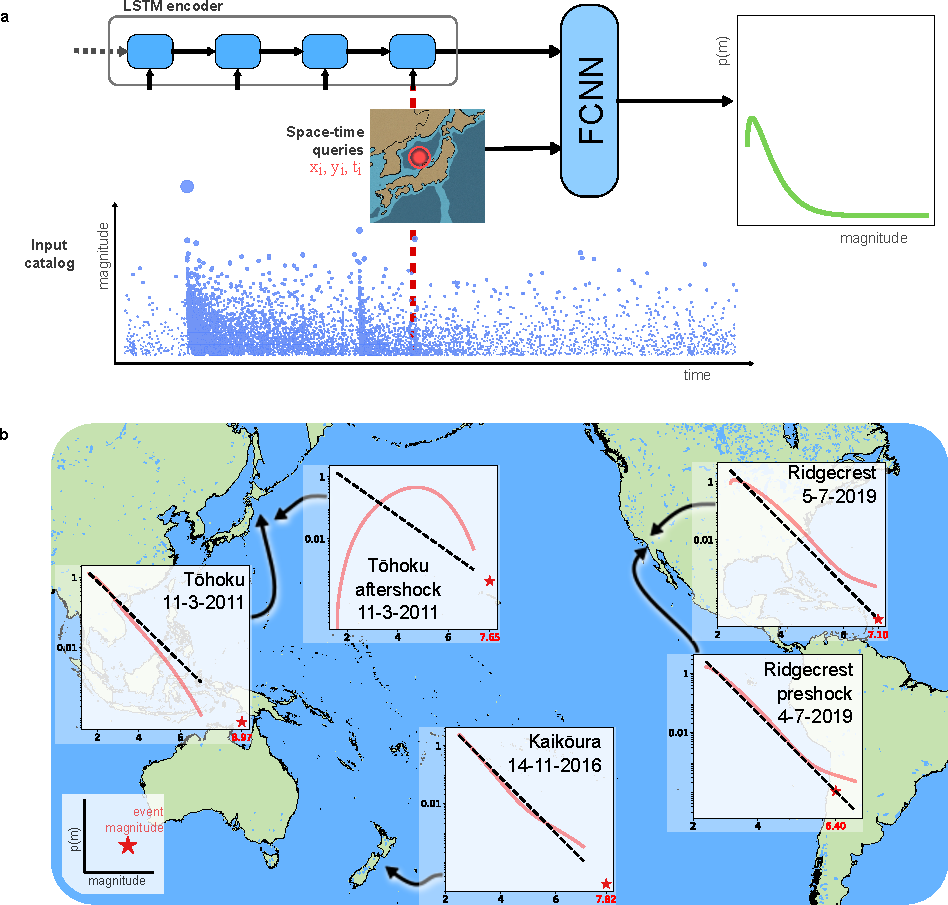
\includegraphics[width=1\textwidth]{figures/intro_fig.pdf}
	\caption{\textbf{a} MAGNET Architecture: A depiction of the task and architecture of the MAGnitude Neural EsTimation model (MAGNET). For each earthquake, seismic history leading up to its occurrence time ($t_i$) is encoded using a Long Short-Term Memory (LSTM) neural network. This encoded history is then concatenated with the timing and location of the earthquake. The combined information is fed into a fully-connected neural network (FCNN) that outputs a probability density function (PDF) representing the possible magnitudes for the given location. \textbf{b} Performance on Major Earthquakes: MAGNET's resulting PDFs for a selection of well-known major earthquakes worldwide. The red curve represents the model's predicted PDF, while the dashed black curve represents the Gutenberg-Richter (GR) magnitude-frequency distribution, a common naive benchmark.  For most earthquakes, the value of the red curve is higher for the actual magnitude (shown by the vertical dashed line), indicating that MAGNET's predictions generally outperform the GR benchmark. Notably, the Tōhoku earthquake exhibits a different behavior.
    }
\label{fig:intro_fig}
\end{figure}

All metrics reported in this work were evaluated over a time span that is not included in training period. The presented metrics demonstrate that our model consistently and significantly outperforms all benchmarks across all test regions, indicating a significant information gain in forecasting earthquake magnitudes prior to their occurrence.
%This finding directly suggests that the seismic system undergoes preparatory processes tailored to the impending event's magnitude before its initiation. Examining these results across multiple catalogs and regions highlights the robustness of our methodology and the generalizability of our conclusion, paving the way for further exploration of earthquake predictability.



\section{Results} \label{sec:results}

% Focusing on existing events within the catalog due to our model's requirement for labeled data, our analysis utilizes the space-time coordinates of earthquakes as input. This necessitates excluding queries about arbitrary spatiotemporal points during training and evaluation, as these processes require knowledge of the true magnitude for each event at its specific location and time. Consequently, the raw output for our analysis consists of the model-generated PDFs of possible magnitudes for each event's time and location. 

Our model, MAGNET, demonstrates the ability to capture the dependence of magnitude distribution on seismic history. Figure \ref{fig:model_output}a showcases the predicted probability density functions (PDFs) $p_{\textbf{x}_i, t_i}(m)$ for 100 randomly sampled events from the Southern California test set. The PDFs exhibit a clear trend: those for higher-magnitude events (warmer colors) are skewed towards larger magnitudes compared to lower-magnitude events (cooler colors). For comparison, the stationary GR distribution, the naive predictor, is presented along the model's results. This result aligns with the expected behavior for earthquake magnitude predictor: dynamically distributing the probability mass for the expected magnitudes. 
Figure \ref{fig:model_output}b depicts the distribution of likelihood scores for the test set across our model (MAGNET), the stationary Gutenberg-Richter (GR) distribution, and a moving window GR approach \cite{gulia_real-time_2019}. Notably, for many high-magnitude events, the model's likelihood scores (red scatter) surpass those of the benchmarks.
To further assess performance in terms of predicted magnitudes, Figure \ref{fig:model_output}c presents the marginal probability density function (PDF) of magnitudes for MAGNET (red) compared to common benchmarks on the Southern California dataset. This figure reveals the general trends predicted by each model and facilitates comparison with the commonly used, stationary GR distribution. Furthermore, Fig. \ref{fig:model_output}c includes histograms of the train and test set magnitudes alongside the marginal PDFs.  We observe that the GR distribution closely follows the train set distribution, as expected for a stationary model.  In contrast, MAGNET aligns well with the test set distribution, suggesting its ability to generalize beyond the training data. Notably, dynamic GR benchmarks, exemplified by the "last 300 events" approach,  while exhibiting a better fit to the test set than the stationary GR, lack the detailed features captured by the model's PDF.


\begin{figure}[h!]
    \centering
    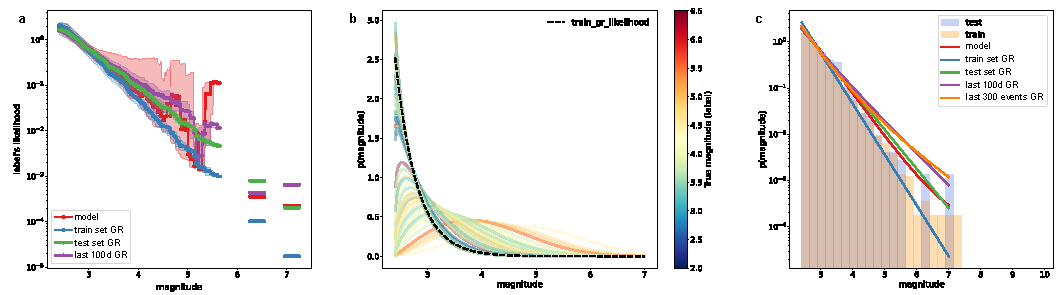
\includegraphics[width=1\textwidth]{figures/raw_results_hauksson.pdf}
    \caption{
        \textbf{Comparison of MAGNET's outputs to benchmarks'}. \textbf{a}, PDFs produced by MAGNET for 100 randomly sampled events from the test set with train set's Gutenberg-Richter distribution (dashed black line). The true magnitude label, i.e. the true magntude of the event in query, is indicated by the color, interpreted by the colorbar at top. \textbf{b}, Likelihoods for returning the magnitude label by MAGNET (red), the 300 events moving window (orange) and the stationary GR (blue dashed line). \textbf{c}, Marginal magnitude distribution, i.e. stationary $p(m)$, produced by MAGNET and common benchmarks for the entire test set. Histograms of the train (and test) set are presented in orange (blue). \neri{c: Is there a more convenient way of showing the two superimposed distributions?}
    }
    \label{fig:model_output}
\end{figure}


Quantification of a model's performance in our scheme will be done by averaging on all log-likelihood scores of the test set, as defined in Eq. \ref{eq:loss_function}. Fig. \ref{fig:metrics}a-c shows the minus mean log likelihood score, $\mathcal{L}$ from Eq. \ref{eq:loss_function}, for MAGNET and chosen common benchmarks, for the three regions tested. It can be clearly seen that MAGNET shows a clear an significant average information gain over every benchmark tested. \neri{Should we mention other benchmarks and refer to the SM?}. 



\begin{figure}[h!]
    \centering
    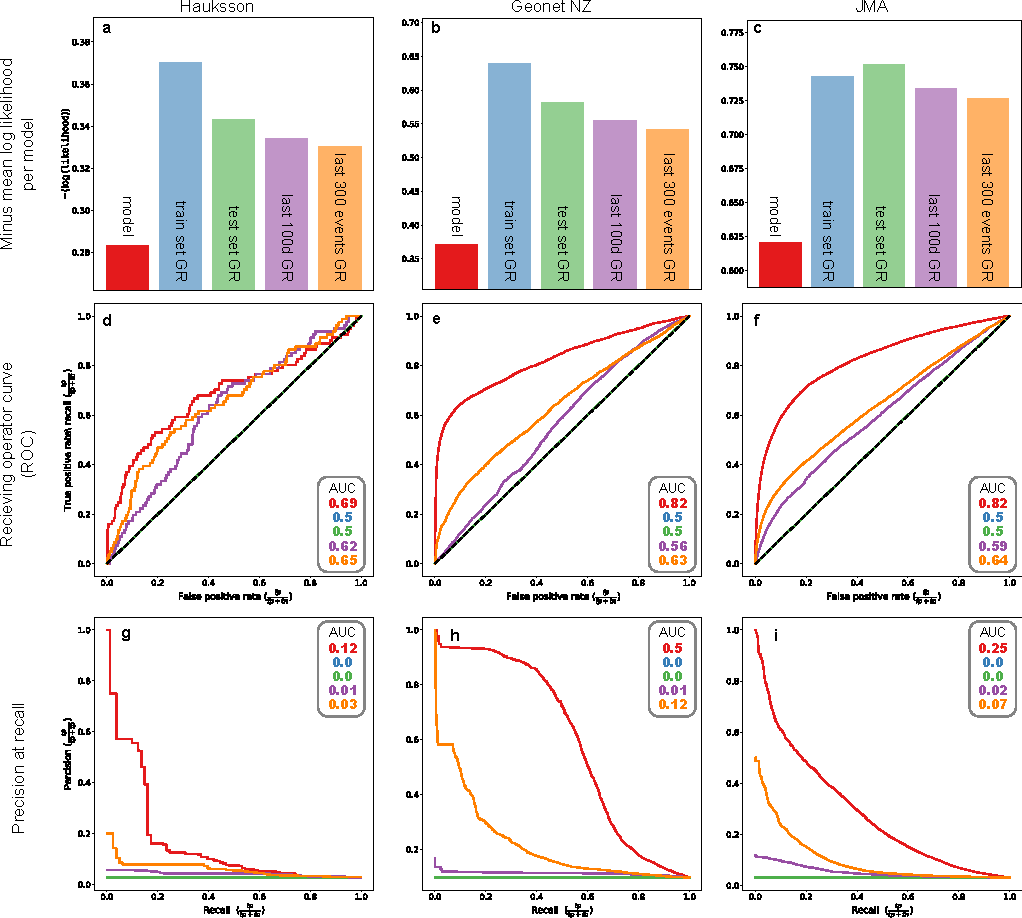
\includegraphics[width=1\textwidth]{figures/combined_batplots.pdf}
    \caption{
        \textbf{Metric scores for the MAGNET model, and common benchmark models. a}, \textbf{b}, \textbf{c}, Minus mean information content of our MAGNET model (red) and other common benchmark magnitude predictors (see labels on bars in the figure). A lower score indicated a better preforming model. \textbf{d, e, f}, Reciever Operating Characteristic (ROC) and \textbf{g, h, i} the interpolated precision-recall (PR) curve for a binary classifier determining the existence of a large ($m>=4$) event. The preformance of such a classifier can be quantified by the area under the curve (AUC), noted in each frame, colorcoded identically to the bar plots. For the AUC metrics, a higher score indicated a better preforming classifier.
        }
        \label{fig:metrics}
\end{figure}

We convert our model to a binary classifier posed with the question: will there be a \textit{large} earthquake in the query space-time coordinates or not? This can easily be done by setting a threshold which defines a "\textit{large}" earthquake, $m_c$ ($=4$ in the examples presented here), then setting examples above that threshold as positive examples and below as negative. The probability of a large event occurring in the query coordinates is given by integrating the output PDF above the threshold, $p=\int_{m_c}^{\infty}p(m')dm'$. Given such binary classifier, it is possible to examine the common binary classifier metrics of area under receiver operator (ROC) curve \cite{Murphy} and under the interpolated precision-recall (PR) curve \cite{buttcher_information_2010} which suit better an imbalanced data set such as ours. \ref{fig:metrics}d-f and g-i show the ROC and interpolated PR curves respectively, for all three regions in examined. The area under the curve (AUC) values are written in the inset of each panel, color coded by the same legend as the bar plots above. It can be seen that throughout all regions MAGNET preforms significantly better than all other benchmarks, indicated by the largest AUC value.

   
    
\begin{figure}[h!]
    \centering
    \includegraphics[width=1\textwidth]{figures/info_over_time_hauksson.pdf}
    \caption{
        \textbf{Analysis of information gain of MAGNET over the benchmark. a,} Information gain of individual events in the Southern California test set. Scattered dots indicate magnitude at event index, colored by the information gain per event (colorbar indicated scale), here warm is an advantage for MAGNET, while cool is an advantage for the benchmark. Secondary horizontal axis (grey) indicates corresponds origin time. Cumulative Information gain (dashed black) and cumulative conditioned information gain (dashed grey) curves are superimposed on the scatter, demonstrating a constantly increasing function. \textbf{b-d}, Information gain (dashed black) and cumulative conditioned information gain (dashed grey) curves for Southern California, New Zealand and Japan test sets, respectively, all three regions examined in this study.\textbf{e-g}, Smoothed instantaneous information gain. Grey cloud shows the standard deviation of the smoothing window. All three curves are predominantly above the zero information gain line (dashed red). \textbf{h-i} Spatial distribution of information gain for all regions in study. Maps show the difference in mean information content per bin, model's advantage is indicated by warm colors, disadvantage by cool colors.
    }
    \label{fig:info_gain_over_time}
\end{figure}
    


The information gain achieved by our model for each event can be quantified by the difference in log-likelihood (LL) between our model's prediction and the baseline GR predictor:
\begin{equation}
    \Delta LL_i = \log{p_{\pmb{x_i}, t_i}^{(MAGNET)}(m_i)} - \log{p^{(GR)}(m_i)}
    \label{eq:information_gain}
\end{equation}
This equation measures the amount of information gained by using our MAGNET model rather than the GR benchmark, for a specific event. Analyzing this quantity per event across the entire test set reveals patterns indicating where and when our model achieves its advantage. Fig. \ref{fig:info_gain_over_time}a shows the test set for Southern California events magnitudes by their running index, colored according to the information gain as defined in Eq. \ref{eq:information_gain}. This time-domain representation allows us to track the cumulative information gain, calculated over the entire test set and displayed as the black dashed line in the figure. The predominantly increasing trend in cumulative information gain suggests that our model is consistently advantageous as opposed to a concentrated advantage in specific periods. Notably, for the Southern California data set, the most rapid information gain occurs during the aftershocks of the two Ridgecrest earthquakes. Surprisingly, even the pre-shock and main shock events demonstrate positive information gains over the GR benchmark, with values of $0.5$ and $1.4, \ \Delta LL$, respectively, albeit these events are typically considered completely unpredictable. This observation leads to a significant corollary: at least some portion of the information gain likely originates from a statistical signal embedded in the event sequence prior to event's occurrence. This point will be further elaborated upon in the discussion section.
\newline

Our analysis reveals a persistent increase in information gain across the test set for all investigated regions (Fig. \ref{fig:info_gain_over_time}b-d). This includes regions previously studied where no information gain was detected using different methods  \cite{ogata_exploring_2018}. Similar domain representations for additional regions can be found in the supplementary material  \neri{TODO: add these colorful plots for NZ and JAPAN to the SM}. Furthermore, the smoothed instantaneous information gain per event, presented in Fig. \ref{fig:info_gain_over_time}e-g, consistently exceeds the threshold for zero information gain marked by the red dashed line.

While the information gain observed in preshock and mainshocks presented above is encouraging, we address a potential concern regarding information gain during high temporal incompleteness periods\cite{stockman_forecasting_2023}. In order to account for the temporal incompleteness artifact, and factor it out of our information gain calculation, we recalculate the likelihood score of each event, $p(m_i)$ , conditioned on the magnitude exceeding a threshold, $\Tilde{m}$:

\begin{equation}
    p \left( m \vert m_i > \Tilde{m} \right) = \frac{p_{\pmb{x}_i, t_i}(m)} {\int_{\Tilde{m}}^{\infty} p(m') ,dm'}
    \label{eq:conditioned_likelihood}
\end{equation}

For our analysis, we set $\Tilde{m} = m_c(t)$, determined dynamically using the maximum curvature method (Weimer and Weiss, 2000) within a window of 150 past and 150 future events. The resulting temporal incompleteness curves are presented in the SM \neri{TODO: add the $m_c(t)$ figure to SM}. After applying the renormalization of Eq. \ref{eq:conditioned_likelihood} the cumulative information gain is recalculated. The result is presented as the grey dashed curved in Fig.  \ref{fig:info_gain_over_time}a, as well as in Fig. \ref{fig:info_gain_over_time}b-d for all three tested regions. Evidently, all conditioned cumulative information gain curves show a steadily increasing trend, supporting the hypothesis that there is information content about the upcoming magnitude in the statistical properties of the catalog, excluding the temporal incompleteness artifact. The mean LL scores of the test set for each data catalog are presented in the supplementary material. \neri{TODO: add conditioned bar plots to SM}.

Beyond the temporal domain, MAGNET also exhibits an advantageous information gain distribution spatially (Fig. \ref{fig:info_gain_over_time}h-j). Each spatial bin's color represents the average log-likelihood difference between MAGNET's predictions and the common GR benchmark (as defined in Eq. \ref{eq:information_gain}, averaged and applied per bin). Warm colors indicate regions where MAGNET performs better. While the advantage in Southern California appears spatially diffuse, both New Zealand and Japan display concentrations of high advantage at the dataset edges, further from the mainland. We hypothesize this is linked to the high local magnitude of completeness, $m_c(x,y)$, in these regions. To address potential artifacts from spatially varying $m_c(x,y)$, we conducted further analysis. We computed local $m_c(x,y)$ per bin and selected only bins with completeness lower than the entire training set's completeness magnitude, $m_c \left( x,y \right)  \leq m_c^{ \left( train \right) }$. We then used these bins to create a minimal dataset and re-ran the model with all previous metrics. As in prior experiments, MAGNET outperformed benchmarks on this minimal dataset. Details and results of this analysis are provided in the supplementary material. \neri{TODO: add these results of minimal data set to the SM}.



% There are two bibliographies in Nature papers. One for the main text, and one for the Methods and Extended Data sections. The numbering is sequential, meaning that the reference section for the Methods and Extended Data section starts after the last number from the main reference section. References should not appear in both sections. Any reference used in Methods or Extended Data that also appears in the main bibliography should *only* appear in the main bibliography.
\let\oldbibliography\thebibliography
\renewcommand{\thebibliography}[1]{%
  \oldbibliography{#1}%
  \setlength{\itemsep}{10pt}%
}
% \bibliography{bibliography}
% \bibliography{bib-article.bib}
\newpage
\bibliography{Magnitude_prediction_paper}

\let\oldthebibliography=\thebibliography
\let\oldendthebibliography=\endthebibliography
\renewenvironment{thebibliography}[1]{
    \oldthebibliography{#1}
    % The number here (34 is an example) is the number of references in the main bibliography, and thus defines the starting number of the first reference in the Methods and Extended Data bibliography.
    \setcounter{enumiv}{34}
}{\oldendthebibliography}

% Figure legends appear after the text, not placed in the text. Do not include the actual image files in the article. Images are submitted as separate files. During the first submission to the journal, you can include the images in the article file for readability, but if you pass the reviews, they will want the images removed from the main article.
\newpage
\unnumbered

\unnumbered
\section{Methods}
\subsection{Neural architecture}
A detailed visual of the model's architecture is presented in Extended Data Fig. \ref{fig:architecture}. The examined catalog is used as an input into three distinct encoding components:
\subparagraph{\textbf{Recent Earthquakes Encoder}} Calculates a set of predefined functions on various past time windows. This encompasses a representation of various statistical properties of the catalog. The result is then used as an input to a LSTM NN. A detailed description of this encoder can be found in past study \cite{zlydenko_neural_2023}. 

\subparagraph{\textbf{Seismicity Rate Encoder}} Computes a rough estimation of the amount of energy released in a given region around the query coordinate, in a given past time window. The result is then used as an input to a LSTM NN. A detailed description of this encoder can be found in past study \cite{zlydenko_neural_2023}.

\subparagraph{\textbf{Event Time Encoder}} Prepares the query time-space coordinates. Time is represented as the time difference from the most recent past event, in seconds. No further processing is done in this encoder.



Outputs of all encoders are concatenated and used as the input to a Fully Connected Neural Network (FCNN). The sizes of layers in the FCNN, as the number of layers themselves, are used as tuneable hyper parameters in order to optimize the architecture by cross validation. A $tanh$ function is used as the activation on the output of every hidden layer, and a $softplus$ as an activation on the output layer. 

\subsection{Loss metric}
To obtain the Probability Density Function of the magnitudes ($p(m)$) for each query coordinates ($\textbf{x}_i, t_i$) we maximize the likelihood presented in Eq. \ref{eq:loss_function}. For our usage we choose $p(\cdot)$ to be a mixture of two stretched and shifted Kumaraswamy distributions \cite{kumaraswamy_generalized_1980}:
\begin{equation}
    p\left( m \right)
    \equiv
    \sum_{j=1,2} \frac{A_j}{\sigma}a_jb_j\left(\frac{m-m_c}{\sigma}\right)^{\left(a_j-1\right)}\left(1-\left(\frac{m-m_c}{\sigma}\right)^{a_j}\right)^{\left(b_j-1\right)}
\end{equation}
Here $a_j, \ b_j$ are the parameters of the Kumaraswamy distribution. $m_c$ is the train set's completeness magnitude. $m_c$ together with $\sigma$ define the support of $p(m)$ to $[m_c, m_c+\sigma]$. $A_j$ is a normalization prefactor, with $j$ the summation index defining the PDF mixture.

\subsection{Definition of benchmark models}
\subparagraph{Last $n$ events} The Gutenberg- Richter (GR) distribution fitted for the past $n$ events. This method follows the method presented in \cite{gulia_real-time_2019} for constructing a b-value time-series. We use the train set's completeness magnitude $m_c^{train}$ to define the GR distribution, and a minimal number of events above $m_c$ ($=10$ in this study). If the minimal number of events above completeness is not fulfilled the window is expanded into the past until the condition is achieved. An attempt to compute $m_c$ per window has been made, though neglected as it showed worse preformance.

\subparagraph{Last $d$ days} The Gutenberg- Richter (GR) distribution fitted for the events in the past $d$ days. This method is identical to the previous method in all but the definition of the window selection.


\subparagraph{Spatially varying Gutenberg Richter}
\subsection{Measurement of temporal incompleteness}




\section*{Data Availability}
This is a required section. Guidelines for data availability: \url{https://www.nature.com/documents/nr-data-availability-statements-data-citations.pdf}.

\section*{Code Availability}
\textbf{Grey's Note} \textit{This is a required section. If your article is about AI or ML, the editor will ask you to make the weights of a trained model available.}


\newpage
\renewcommand\refname{Methods References}
\begin{thebibliography}{10}
\bibitem{zlydenko_neural_2023}
Zlydenko, O. et al. A neural encoder for earthquake rate forecasting. Sci Rep 13, 12350 (2023).
\end{thebibliography}


\newpage
\section*{Acknowledgements}
Acknowledgements should be brief, and should not include thanks to anonymous referees and editors, inessential words, or effusive comments. A person can be thanked for assistance, not “excellent” assistance, or for comments, not “insightful” comments, for example. Acknowledgements can contain grant and contribution numbers.

\section*{Author Contributions}
Author Contributions: Authors are required to include a statement to specify the contributions of each co-author. The statement can be up to several sentences long, describing the tasks of individual authors referred to by their initials. See the authorship policy page for further explanation and examples.


\section*{Author Information}
\textbf{Grey's Note} \textit{Two things are required in this Author Information section: (1) A statement about competing interests. I have no advice about what constitutes a competing interest, you will have to read about it and make your own decision. (2) A clear statement about who to contact with question about the paper. An example is below.}
% For example:
% The authors declare no competing interests. Please contact either the first author (Grey Nearing; \href{mailto:nearing@google.com}{nearing@google.com}) or Avinatan Hassidim; \href{mailto:avinatan@google.com}{avinatan@google.com}) for correspondence and requests, including questions regarding reprints and permissions.


\newpage
\section*{Extended Data}
\begin{enumerate}
    \item Table: scores of all metrics - \textbf{should I add this??}
    \item Detailed architecture? - \textbf{should I add this??}
    \item Colorful PDF examples for NZ and Japan
    \item Marginal distributions for NZ and Japan
    \item Colored scatter magnitude vs index, NZ and Japan - \textcolor{red}{\textbf{Done}}
    \item $m_c(t)$ for all three regions -  - \textcolor{green}{kind of finished plot, not sure}
    \item Bar plots of conditioned $<LL>$
    \item Spatial $m_c(x, y)$ and low $m_c(x, y) \leq m_c^{train}$ bins
\end{enumerate}

\newpage
\begin{figure}
    \centering
    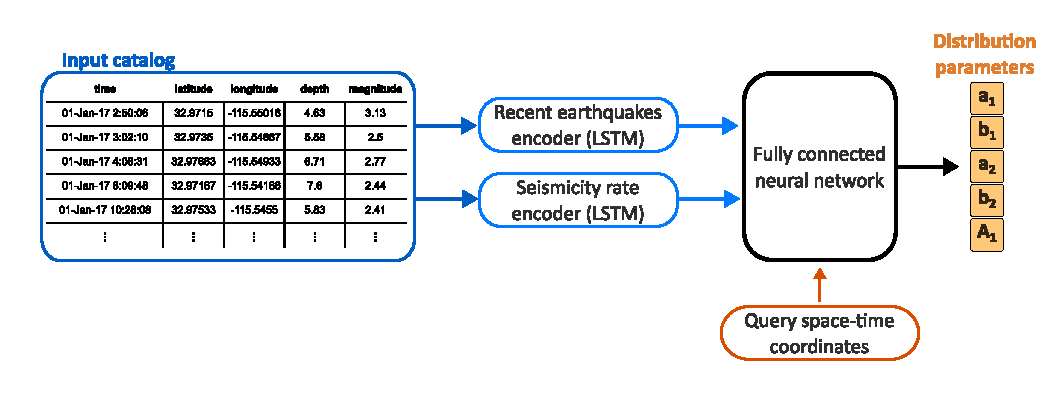
\includegraphics[width=1\textwidth]{figures/detailed_architecture.pdf}
    \caption{\textbf{MAGNET architecture.} Described in detail in the methods section.}
    \label{fig:architecture}
\end{figure}

\newpage
\begin{figure}[h!]
	\centering
        \includegraphics[width=1\textwidth]{figures/info_gain_scatter_NZ_and_Japan.pdf}
	\caption{
            \textbf{Information gain over time domain for New Zealand and Japan data sets.} This figure presents results for the data sets not displayed in Fig. \ref{fig:info_gain_over_time}a. \textbf{a} Entire test set of New Zealand and a selected time span (\textbf{b}) focusing on the 2016 Te Araroa earthquake and the 2016 Kaikōura earthquake. \textbf{c} The entire Japan data set and a focused time span \textbf{d} of the 2011 Tōhoku earthquake and some of its aftershocks.
         }
\label{fig:intro_fig}
\end{figure}

\newpage



\textbf{Grey's Note} \textit{You get up to 10 items in the Extended Data section. All Tables and Figures should be enumerated as "Extended Data Figure 1", "Extended Data Table 1", etc. These must also be referenced the same way in the text. Extended Data tables and figures may be referenced in the main article and/or in the Methods section. I am doing the in-text references to these ED items manually, instead of trying to override the table numbering schemed in Latex. Please update this template to automate that process if you feel like doing that.}

\textit{You can use Latex formatting for tables, but the journal will eventually require that your tables be submitted as images. Yes, this also struck me as unusual.}

\textit{Each ED figure should be on a separate page.}

\textit{Finally, this note is here in the ED section, but in your paper, the ED section should not have any text except figure and table captions/legends.}

\end{document}
